

\section{Introduction}

This section largely remains the same as in the Note 103~\cite{JCN:103}.
However, with the new available data from LEP, the JADE data 
obtained more importance as a case of successful data preservation.




\section{JADE data}
\label{sec:data}
The JADE data is stored at MPCDF, can be accessed via various protocols, and is available as open data
(Section~\ref{sec:opendata}).

\subsection{Data formats}
The JADE data, the real data after the two data reduction steps~\cite{JCN:38,JCN:43} and the Monte Carlo data, are
organised in the framework of the data management system BOS~\cite{Blobel:BOS} (version of 1979), which was introduced in the
1970s for the online and offline data flow of the high energy physics experiments at DESY. Two further formats are used
for the summarised events: ZE4V~\cite{JCN:99}, which is independent of BOS, and the BOS-based TP format~\cite{JCN:102}, whose
files have not been recovered. The original raw data were copied from the IBM computers of DESY in 1997 and converted
with the FPACK program into a machine independent word format (format \texttt{B32}), in which the data of the
banks are copied word by word as 32-bit patterns; the program \texttt{fptobos} converts these files back into BOS banks.

\subsubsection{BOS records}
In BOS all event data and analysis information are structured in banks of variable length. A JADE event record is a
dynamically arranged set of standardised BOS banks that represent the subsystems of the detector (the raw jet chamber data,
the lead glass ADC counts, \dots) or results of the event analysis (the tracks of the pattern recognition, the lead glass
clusters, \dots); a complete event has about two dozen banks. A bank is identified by a name and a number. It has a header
of four 32-bit words (the bank name, the bank number, a pointer to the next bank with the same name and the number of data
words) followed by the data. Some of the most important banks are:
\begin{itemize}
\item \texttt{JETC}, the raw jet chamber data~\cite{JCN:23}: a bank of 16-bit words. Its first part has pointers to the first
hit of each of the 96 drift cells, in the second part every hit is a sequence of four 16-bit words (the wire and the hit number,
the pulse amplitudes at the two ends of the wire and the drift time).
\item \texttt{PATR}, the tracks of the pattern recognition~\cite{JCN:12}, with the curvature, the fit type and parameters and the
fit quality of every track as 32-bit integers and floating point numbers, and \texttt{JHTL}, the hit label bank~\cite{JCN:21},
with two 16-bit words per hit that relate the hits to the tracks. The results of different steps are marked by the bank number,
e.g.\ \texttt{PATR/10} is usually the result of the standard pattern recognition.
\item \texttt{ALGL}, the raw lead glass data (ADC counts and channel numbers of the hit blocks), \texttt{ALGN}, the pulse heights
in MeV sorted by the clusters, and \texttt{LGCL}, the final lead glass clusters with their energies, directions, shower profiles
and track correlations~\cite{JCN:14D}.
\end{itemize}
The banks are compact mixtures of 16-bit and 32-bit integers and of floating point numbers, because at the time of PETRA
the data acquisition and processing were dominated by the need to save memory. For the present machines this layout is
problematic: the access to a data word or to a bit of a bank depends on the byte order of the machine (Section~\ref{sec:endian}).

\subsubsection{ZE4V records}
The ZE4V format~\cite{JCN:99} is a compact format of the reconstructed events, which was introduced by a group of the
collaboration for the studies of multihadronic final states. A ZE4V record can be handled without BOS (the software that
produces and reads it works inside the BOS environment) and is a mixture of 16-bit and 32-bit words. It starts with a header
with the structure of the record and global properties of the event. The particle section follows, with the measured
quantities of the reconstructed charged particles and photons: every particle begins with a general part (the four-momentum,
the charge, \dots), followed by a part specific to charged particles (e.g.\ the number of inner detector hits or the point of
closest approach of the track) or to neutral particles (e.g.\ the uncorrected cluster energy and the number of lead glass blocks
of the cluster). The record also has a Monte Carlo section with the four-vectors of the initial parton or hadron configuration of
a simulated event. The ZE4V records are written by the program \texttt{ze4v} (Section~\ref{sec:ze4v}).

\subsection{Data preprocessing history}
The data passed through a multi-level trigger and filters: the first level trigger T1 (an energy trigger on the fast analogue
signals of the lead glass), the track trigger T2 of the jet chamber and the third level trigger T3 on the drift data of the muon
filter. Online filters rejected the background events (cosmic rays, beam-gas interactions, electronic noise), and the accepted events
went from the data acquisition computers (NORD-10S and NORD-50 of Norsk Data~\cite{Wiki:Nord}) to the IBM mainframes of DESY~\cite{Wiki:IBM370}.
Both the online and the offline flow of the data were managed within BOS. After a general reformatting the data were passed through the
two reduction steps (REDUC1~\cite{JCN:38} and REDUC2~\cite{JCN:43}) that enrich the fraction of the signal events with cuts partly based on the
reconstructed events (the banks \texttt{PATR} and \texttt{LGCL} of the Supervisor).

\subsection{Calibration Files}
\label{sec:calfiles}

The calibration constants are kept in the ASCII files \texttt{aupdat1}, \texttt{bupdat0} and
\texttt{bupdat1} and in their binary counterparts \texttt{aupdat1.b}, \texttt{bupdat0.b} and
\texttt{bupdat1.b}, which are the files read by the programs. The calibration scheme is described in
``The JADE Calibration Scheme''~\cite{JCN:68}. The records of the files
are read by the routine \texttt{KLREAD}, which copies the constants valid for the time of the event
into the common block \texttt{/CALIBR/}.

\subsubsection{Calibration constants were not applied on little-endian machines}

While checking why the muon chamber outlines were missing in the event display and why the muon
analysis reported \texttt{NO CALIBRATION FOUND}, it was found that on a little-endian machine the
routine \texttt{KLREAD} did not apply \emph{any} record of the calibration files, not only the muon
chamber constants (\texttt{MUCA}). The cause is the identification of the records. \texttt{KLREAD}
applies a record only if the bank name in the second word of the record is equal to one of the
Hollerith constants of its list (\texttt{4HMUCA}, \texttt{4HLGMA}, \texttt{4HTAGS}, \dots,
\texttt{IF(NAMEBN.EQ.NAME(I))}). The numbers of the binary files are converted by the Fortran
runtime (\texttt{GFORTRAN\_CONVERT\_UNIT=big\_endian} etc.), but the name is stored in the same kind of
integer word and has to agree with the constant of the program. The binary files that were shipped
had the names in the byte order of the big-endian machine on which they were produced, so on
little-endian hosts no name matched and every record was skipped silently. This was seen with a
debugger: the code that applies a bank was never reached while 1151 records were read, \texttt{/CALIBR/}
stayed empty (\texttt{NVERSN=0}, \texttt{IZOEP1=IZOEP3=0}), and the same program with the name list
byte-swapped in memory loaded the muon calibration (\texttt{NVERSN=4}, \texttt{IZOEP1=1960},
\texttt{IZOEP3=2150}).

\subsubsection{Corrected binary files}

The ASCII files, which were not changed, were converted again with the program \texttt{conv} on a
little-endian machine (Section~\ref{sec:calconv}). Two sets of the files are present in the source tree:
\begin{description}
\item[\texttt{jadesoft/cal}] the original binary files, made on a big-endian machine (not modified).
\item[\texttt{jadesoft/cal2026}] the ASCII files and the binary files converted for little-endian machines.
\end{description}
The build (\texttt{jadesoft/CMakeLists.txt}) installs the set that fits the byte order of the host
into \texttt{share/JADESOFT/cal}, from where all tests and scripts take the files: \texttt{cal} on
big-endian and \texttt{cal2026} on little-endian machines. The choice can be forced with
\texttt{-DJADE\_CAL\_DIR\_NAME=cal} or \texttt{cal2026}.

The muon calibration needed one more correction. Some \texttt{INTEGER*4} variables of the muon
calibration (\texttt{NFRAMS}, \texttt{NCHAMS}, \texttt{IFCIND(1..6)} in \texttt{jademus/cmucalib.for})
are \texttt{EQUIVALENCE}d to pairs of half-words, which \texttt{conv} puts in the order of the host. These
words are completed by exchanging the two halves of the word (script
\texttt{jadesoft/cal2026/fix\_overlay\_words.py}, Section~\ref{sec:calconv}). Without this step the
muon region routine stopped with \texttt{TOO MANY MU PLANES} (\texttt{NFRAMS} and \texttt{NCHAMS} were
wrong), with it the values are \texttt{NFRAMS=82}, \texttt{NCHAMS=634}. The other banks with half-word
constants were checked as far as possible: \texttt{LGMA}, \texttt{TAGS} and \texttt{JTPL} are used as
pure half-word arrays; \texttt{LGST}, \texttt{SPTG} and \texttt{TAGF} are empty for the test data and
could not be checked.

\subsubsection{Effect and tests}

With the corrected files the banks \texttt{MUCA}, \texttt{LGMA}, \texttt{JTPL}, \texttt{JTAB},
\texttt{TOFC}, \texttt{DEDX}, \texttt{RVTX} and \texttt{ZCAL} are loaded into \texttt{/CALIBR/} for the
test data, with plausible values (e.g. the half-word constants of \texttt{LGMA} and \texttt{JTPL} are
in the ranges 0--15160 and 0--1348). The reconstruction of the test sample with the Supervisor
was compared bit by bit with the result obtained with the original files: only the bank \texttt{ALGN}
differs, it contains zeros without and numbers with the calibration, all other banks are identical.
Switching on the calibration groups of the other banks does not change the result of this
reconstruction. The muon filter views of the event display (\texttt{RC1}, \texttt{ZXC1}, \dots) now
show the outlines of the muon chambers, which were missing before (the test event has no muon hits).

With the corrected files all 35 tests of the test suite pass in the 64-bit builds with the GNU, Intel (\texttt{ifx}) and NVIDIA (\texttt{nvfortran}) Fortran compilers, including the event display tests.

The test suite checks the calibration at two levels. The tests \texttt{CALIB\_NAMES\_aupdat1},
\texttt{CALIB\_NAMES\_bupdat0} and \texttt{CALIB\_NAMES\_bupdat1} (\texttt{test/src/calcheck.f}) read the
installed binary files in the way of \texttt{KLREAD}, count the records whose name is recognised and fail if
a record is not recognised or if no \texttt{MUCA} record is present; they fail for the original files on a
little-endian machine (0 of 3131 records recognised). The three event display tests fail if the muon
analysis reports \texttt{NO CALIBRATION FOUND}, i.e.\ if the constants were not used by a running program.

\subsubsection{Muon system}

The muon chamber calibration is now available, but the muon system remains largely unsupported.
In the Monte Carlo the routines \texttt{MURTNE}, \texttt{MUORDR} and \texttt{MUCONM} are dummies
(as stated in ``A Guide to the Resurrected JADE Data and Software''~\cite{JCN:103}, the libraries of the muon Monte Carlo of the thesis~\cite{Bowdery:1982thesis} could not be retrieved), so no muon
chamber hits are simulated. In the Supervisor the muon analysis step is skipped
(level 8 is marked ``unused'' in \texttt{main2016/superv/user.f}). The documentation of the
muon system is in the JADE Computing Notes on the muon graphics commands~\cite{JCN:52}, the muon Monte Carlo at DESY~\cite{JCN:55}, the JADE Monte Carlo~\cite{JCN:67} and the muon track finding algorithm \textsc{mutana}~\cite{JCN:82}; they are scanned images, available on the CERN Open Data Portal
(Section~\ref{sec:opendata}), where each note has a record number.


\subsection{Open data}
\label{sec:opendata}

The JADE data and software are published on the CERN Open Data Portal (\url{https://opendata.cern.ch}, experiment
JADE). The portal contains:
\begin{description}
\item[The data.] One dataset with the raw electron-positron collision data of the JADE detector at the PETRA
accelerator of DESY~\cite{OpenData:JADE} (record 26999, published 2024, license CC0-1.0). It contains all data
recorded from 1979 to 1986 with collision energies from 12 to 46.7~GeV, in the raw (FPACK) format as they were
recovered from the archives: 2862 files with a total size of about 620~GB. The files are named as the files of
the original tapes (\texttt{JAD001/file001}, \dots; the data of one tape directory are listed in an index file
\texttt{JAD001\_file\_index.json}) and are accessed with the XRootD protocol~\cite{Dorigo:XRootD} from the CERN storage
(\texttt{root://eospublic.cern.ch//eos/opendata/jade/datasets/jadetapes/}). The data file used by the test suite of
this repository, \texttt{test/jadetapes/JAD073/file006}, has the same naming. The raw data are converted to BOS
banks with \texttt{fptobos} and processed with the reconstruction; the portal has no Monte Carlo samples, they
are generated with the programs described in this note.
\item[The software environment.] The JADE virtual machine image (record 26000~\cite{OpenData:JADEVM}, CentOS~7,
VirtualBox format, 2.8~GB) with the reconstruction software of 2016, and the guides ``Getting started with JADE
Open Data'' (installation of this software in a container with Docker or Podman and the test with
\texttt{jadeinstall.sh} and \texttt{jadetest.sh}), ``JADE Virtual Machines: how to install'', ``Understanding
JADE software'' and ``Understanding JADE MC generation''. The guides refer to the repository of this software
and to the container images that were current at the time; the images and the commands of the present version are
described in Section~\ref{sec:build} and in the environment description above.
\item[The documentation.] The scanned JADE computing notes (117 records at the time of writing), the logbooks
(21 records), the author lists of the collaboration and of the preserved data, and the page about the experiment
(\url{https://opendata.cern.ch/docs/about-jade}).
\end{description}
The portal gives access to the unprocessed data only; the preserved software, with the calibration files and the tests
described in this note, is what makes them usable.

\subsection{The luminosity table}
\label{sec:lumi}

The integrated luminosity of the data is not part of the event data; it is tabulated by run period in the directory
\texttt{jadesoft/info} of the repository:
\begin{description}
\item[\texttt{lumi.dat}] the table of the luminosity of the barrel luminosity monitor, integrated over consecutive runs with
the same beam energy (run periods). Each line has the first and the last run of the period, the beam energy in GeV, the
integrated luminosity and its error (format \texttt{(2(I5,3X),F6.3,2E14.6)}); the unit is not written in the file (it is
presumably nb$^{-1}$). The numbers were transferred by hand from a historic printout of the program
\texttt{TAKLUMI} by J.~Olsson. The file \texttt{lumi.dat.ori} is that transcription; \texttt{lumi.dat} has the tabulators
replaced by blanks, the zero entries brought to the format of the others and the missing run periods 540--564 and
581--591 added from the first page of the printout (with four digits of accuracy).
\item[\texttt{jaderuns.dat}] the overview of the beam energy against the data taking period and the run period (year, dates,
first and last run, beam energy, period number), in a format that is easier to process than \texttt{jaderuns.dat.ori}, with two
lines corrected in 1985.
\item[\texttt{shutdown.dat}] the shutdown periods of the accelerator.
\item[\texttt{taklumi.f}, \texttt{taklumi.dat}, \texttt{README}] the historic source of the program \texttt{TAKLUMI}, an example
of its input and the description of the files.
\end{description}
The program \texttt{taklumi} (source \texttt{jtuple/src/taklumi.f}, installed with the other programs) sums the luminosity.
It reads the file \texttt{lumi.dat} from the working directory and the first and the last run number from the standard
input (the file \texttt{taklumi.dat} gives examples of run ranges), and prints the luminosity of each run period, the
sum for the run range and the sums per centre-of-mass energy range, with the errors; the histograms of the integrated
luminosity are written with HBOOK. The luminosity of a selection of the data is the sum over the run periods of the runs
that it contains.

\section{JADE Program Libraries}

\subsection{Location}
The source code of the software is in the \texttt{jadesoft} directory of the repository
\url{https://github.com/andriish/JADE} (Section~\ref{sec:build}); the installed software is in the install
prefix of the build (\texttt{installed<toolchain><bits>} in the repository directory by default): the programs in
\texttt{bin}, the libraries in \texttt{lib} (\texttt{lib64} on Fedora and CentOS), and in \texttt{share/JADESOFT} the
calibration files (\texttt{cal}, Section~\ref{sec:calfiles}), the example input cards of the programs and the CMake
package configuration.

\subsection{Organisation}
The directory \texttt{jadesoft} contains the software in its original form and the current versions:
\begin{itemize}
\item \texttt{src2016} the libraries of the current version (\texttt{boslib} BOS, \texttt{jadegs} reconstruction
supervisor and calibration, \texttt{jmc} and \texttt{jade56} detector simulation, \texttt{patrecsr} and
\texttt{vertex} pattern recognition, \texttt{jademus} muon analysis, \texttt{tagg} tagging system, \texttt{toflib} time of
flight, \texttt{grafix} and \texttt{interface} event display, \texttt{zlib} ZE4V, \texttt{source} common routines,
\dots), compiled into static libraries;
\item \texttt{main2016} the main programs \texttt{mcjade}, \texttt{superv}, \texttt{ze4v} and \texttt{jadez};
\item \texttt{util2016} the utilities: the calibration file converters (\texttt{ccal}), the old Monte Carlo generators
(\texttt{mcgen}) and the programs that read the ZE4V data (\texttt{zread});
\item \texttt{job2016} the example steering scripts and data of the programs; \texttt{cal} and \texttt{cal2026} the
calibration files;
\item \texttt{src}, \texttt{src0}, \texttt{main}, \texttt{job}, \texttt{util} the original and pre-2016 sources, which
are kept for reference and are not used in the build.
\end{itemize}
The other programs of the repository are in their own directories: \texttt{convert} (Monte Carlo events to the JADE
format), \texttt{fptobos} (raw data to BOS), \texttt{jtuple} (ntuples with the QCD observables) and \texttt{h2root}
(HBOOK to ROOT).

\subsection{Installation}
The installation is done with the scripts of Section~\ref{sec:build}:
\begin{lstlisting}
sh jadeinstall.sh [--bits=32|64] [--toolchain=NAME] [--prefix=/path]
sh jadetest.sh    [--bits=32|64] [--toolchain=NAME] [--prefix=/path]
\end{lstlisting}
The first script builds and installs the projects in the order \texttt{jadesoft}, \texttt{convert}, \texttt{jtuple},
\texttt{fptobos}, \texttt{h2root}, and the second, with the same options, builds and runs the test suite. Everything is installed under the
prefix \texttt{installed<toolchain><bits>} unless \texttt{--prefix} is given. The dependencies are described in
Section~\ref{sec:deps}; the simplest way to get them is a container image (see the description of the environment below).

\section{Handling the main programs}

The main programs are run in a directory that contains their input files; the steering input is a card file
(the format of the \texttt{FFREAD} package of CERNLIB: one key and its value per line, comments start with \texttt{C}) that
is given to the standard input of the program, e.g.
\begin{lstlisting}
cat mcjade1.card | mcjade
\end{lstlisting}
The names of the input and
output files, the options and the numbers of the events are set in the card; examples of the cards for every
program are in \texttt{share/JADESOFT} and in \texttt{test/cards}. The byte order of the files has to be set for the
Fortran runtime (Section~\ref{sec:endian}).

\subsection{mcjade}
The program \texttt{mcjade} is the simulation of the response of the JADE detector (tracking in the jet and the
vertex chambers, the lead glass calorimeter showers with their smearing and absorption, the time of flight, the
tagging system; no muon system, Section~\ref{sec:calfiles}).
\begin{description}
\item[Input] the file with the four-vectors of the generated events in the CPROD format (card key \texttt{MCVECT}),
produced by the old generators or by \texttt{convert} (Section~\ref{sec:convert}); the date of the configuration of the
detector (\texttt{YEAR}, \texttt{MONTH}, \texttt{DAY}), which selects the detector hardware of the data period, the
tracking options (\texttt{SMEAR}, \texttt{CONVERT}, \texttt{ABSORB}, \texttt{SHOW3D}, \texttt{VERTEX}) and the first and
last event.
\item[Output] a BOS file with the simulated detector data (\texttt{MCBOS}), optionally a print out of the banks in
text form (\texttt{MCBANK}) and control histograms (\texttt{MCHIST}); the output file is in the native byte order.
\end{description}

\subsection{superv}
The program \texttt{superv} is the JADE Supervisor, the reconstruction of the events of the real data and of the
simulation.
\begin{description}
\item[Input] the BOS file with the raw data (from \texttt{fptobos}) or with the simulated data from \texttt{mcjade}
(card key \texttt{MCBOS}), the calibration files (\texttt{AUPDAT0}, \texttt{BUPDAT0}, \texttt{BUPDAT1}: the
installed \texttt{aupdat1.b}, \texttt{bupdat0.b}, \texttt{bupdat1.b}), the flags that select the groups of the
calibration constants that are read (\texttt{MUCA}, \texttt{LGMA}, \dots) and the reconstruction options
(\texttt{ZSRFTV}, \texttt{VTXFIT}), and the first and last event.
\item[Output] a BOS file with the reconstructed events: tracks, vertices, lead glass clusters and the other banks
(\texttt{SVBOS}), a text print out of the selected banks for the levels of the processing (\texttt{SVBANK}, the banks are
chosen with \texttt{LEVEL1\dots LEVEL7}), control histograms (\texttt{SVHIST}) and the file \texttt{superv.stat} with the
state of the random number generator. All units except the BOS input of the program are big-endian.
\end{description}

\subsection{ze4v}
\label{sec:ze4v}
The program \texttt{ze4v} compresses the reconstructed events into the ZE4V format of the analyses.
\begin{description}
\item[Input] the BOS file written by \texttt{superv} (card key \texttt{SVBOS}), the number of events to read and to
skip (\texttt{EVTREAD}, \texttt{EVTSKP}), the selection flags (\texttt{SELECT}, \texttt{MSELCT}, \texttt{ESELCT}) and the
calibration files.
\item[Output] the file with the compressed events in the ZE4V format (\texttt{ZE4V}), optionally a BOS file with the full
events (\texttt{ZBOS}) and a text print out of the selected banks (\texttt{ZBANK}, \texttt{CONT}).
\end{description}
The ZE4V files are read by the program \texttt{jzread}, which writes an HBOOK ntuple, and the ntuples are processed
by \texttt{jtjob} (directory \texttt{jtuple}) and converted to ROOT files with \texttt{h2root}.

\subsection{jadesim}
\texttt{jadesim} is the steering job of the old simulation that ran the whole chain for one sample: the event generation
(with the cards \texttt{GEN.CARD} or \texttt{GEN\_JT63.CARD}, and the data files of COJETS), the tracking with
\texttt{mcjade} (\texttt{MC.CARD}), the smearing and the reconstruction with \texttt{superv} (\texttt{SV.CARD}) and the
compression with \texttt{ze4v} (\texttt{ZE.CARD}); the output of every step was written into a directory of the job. The
job was a script of the IBM and the LoadLeveler batch systems, which is no longer supported, and it is obsolete:
the Monte Carlo events are generated by external generators and converted with \texttt{convert}, and the chain is run
by the test suite and the programs above. The script is kept for the correspondence between the centre-of-mass
energy and the configuration of the detector that its cards use:
\begin{center}
\begin{tabular}{|c|c|c|c|c|}\hline
Sample & CMS energy, GeV & Year & Month & Day \\\hline
14  & 14.0 & 81 & 07 & 17 \\
22  & 22.0 & 81 & 06 & 17 \\
35a & 34.6 & 82 & 05 & 17 \\
44  & 43.8 & 85 & 05 & 17 \\
38  & 38.3 & 85 & 10 & 01 \\
35b & 35.0 & 86 & 05 & 17 \\\hline
\end{tabular}
\end{center}
The year, the month and the day are the values of the keys \texttt{YEAR}, \texttt{MONTH} and \texttt{DAY} of
\texttt{mcjade}.

\subsection{jadez}
The program \texttt{jadez} is the interactive event display (Section~\ref{sec:display}).
\begin{description}
\item[Input] the name of a BOS file (asked in the dialog), the calibration file in the working directory (the
installed \texttt{aupdat1.b}, copied to \texttt{F11LHO.AUPDAT1}), the help data set (\texttt{F22BOW.HELP.DATASET}) and
the commands of the display, typed or read from the standard input and ended with \texttt{END}; the window is opened
on an X11 display.
\item[Output] the pictures in the window and the hardcopies (command \texttt{H}) in the PostScript files
\texttt{JADE.nnn.ps} (the display tests convert them to PNG); the text commands print on the terminal.
\end{description}

\section{Utility programs}



\subsection{QCD Event Generator Package and CPROD Interface}
\label{sec:convert}
The JADE detector simulation \texttt{mcjade} takes the generated events in the format of the JADE Monte Carlo
(CPROD) and the old generators of the historic JADE productions write this format directly. The directory
\texttt{convert} contains the program \texttt{convert\_hepmc\_to\_jade}, which converts the events of modern
generators into CPROD files. It is based on the format conversion example of HepMC3~\cite{Buckley:2019xhk}
(HepMC3 3.1 or newer is needed) and is run as
\begin{lstlisting}
convert_hepmc_to_jade -i hepmc3 -o jade input.hepmc output.cprod
\end{lstlisting}
The input can be in any format that HepMC3 reads: HepMC3 and HepMC2 ASCII, HEPEVT, LHEF~\cite{Alwall:2006yp}, ROOT files, compressed
files or the plugins of HepMC3; the same program also converts between these formats.

For each event the writer fills the CPROD record with the event number, the beam energy, the flavour of the
primary quark pair (the hard quark--antiquark pair with an energy sum of more than half of the beam
energy), all particles with their four-momenta, masses, charges (from the PDG identification codes,
\texttt{AtlasPID.h}~\cite{Verbytskyi:AtlasPID}, which implements the numbering scheme of the Particle Data Group~\cite{PDG:MCnumbering}), and the links of the particles to the partons they come from, and the final-state particles
(status 1, without neutrinos, which the detector does not see) with their names, production vertices and the
numbers of charged and neutral particles. The converted file is then passed to the detector simulation, the
reconstruction and the analysis programs, which is the processing chain of the test suite.

Because the interface is HepMC3, events of many generators can be used for the JADE detector simulation, as
all of them can write HepMC events. The test suite uses Pythia 8~\cite{Bierlich:2022pfr}; other generators that can
write HepMC events and are suitable for $e^+e^-$ annihilation at the PETRA energies are, for example,
Sherpa~\cite{Bothmann:2019yzt,Sherpa:2024mfk}, Herwig 7~\cite{Bellm:2015jjp,Bewick:2023tfi} and
WHIZARD~\cite{Kilian:2007gr}. Only the conversion of Pythia 8 events is tested here; the choice of the generator
settings for the JADE data (the beam energies, the hadronisation parameters and the smearing) is described
in the guide ``Understanding JADE MC generation'' of the open data portal (Section~\ref{sec:opendata}).



\subsection{Example Program for Processing ZE4V Data}


\subsection{Conversion tool for JADE calibration files}
\label{sec:calconv}

The program \texttt{conv} (source \texttt{jadesoft/util2016/ccal/conv.f}, installed with the other
programs) converts an ASCII calibration file into the binary format. It has fixed file names: it reads
\texttt{aupdat1} from the current directory and writes \texttt{aupdat1.b}, and the information on every
record is printed on the standard output. The bank name is read from the text into an integer
(\texttt{A4} format), so the name word has the byte order of the machine that runs the program;
the output unit has to be big-endian, as the programs read it. The binary files for a little-endian
machine were made as follows (the files of \texttt{jadesoft/cal2026}):
\begin{lstlisting}
export GFORTRAN_CONVERT_UNIT=big_endian    # F_UFMTENDIAN=big for Intel
mkdir work; cd work
cp ../jadesoft/cal2026/bupdat0 aupdat1     # conv always reads the file aupdat1
conv > conv.bupdat0.log                    # writes aupdat1.b
mv aupdat1.b ../jadesoft/cal2026/bupdat0.b
\end{lstlisting}
and the same for \texttt{aupdat1} and \texttt{bupdat1}. The half-word constants of the ASCII files are
packed by \texttt{conv} two per word in the order that the program needs on a little-endian machine,
with one exception: the muon calibration (bank \texttt{MUCA}, layout in \texttt{jademus/cmucalib.for})
has 4-byte integer variables that are \texttt{EQUIVALENCE}d to a pair of half-words (\texttt{NFRAMS},
\texttt{NCHAMS}, \texttt{IFCIND(1..6)}, i.e. the words 20, 390 and 4155--4160 of the muon calibration
array). In a second step the two halves of these words are exchanged:
\begin{lstlisting}
python3 jadesoft/cal2026/fix_overlay_words.py in.b out.b
\end{lstlisting}
With this step the muon
constants read by \texttt{KLREAD} are correct (\texttt{NFRAMS=82}, \texttt{NCHAMS=634},
\texttt{IZOEP1=1960}, \texttt{IZOEP3=2150} in \texttt{/CALIBR/}). The other banks with half-word
constants were not checked for such overlays. The original files
(\texttt{*-ori.gz}) are converted after \texttt{gunzip}. The conversion logs were stored as
\texttt{conv.*.log.gz}. The result can be checked with the test \texttt{CALIB\_NAMES} of the test
suite or directly with \texttt{calcheck file.b} (with the same environment variable).

\section{Reactivation of the JADE software}




\section{Remaining tasks}
This section of the original note is obsolete.

The straightforward modifications considered in the original note
\begin{itemize}
\item As of 2026, it makes sense to
have the routines for event analysis that use external libraries, e.g. ROOT~\cite{Brun:1997pa,Antcheva:2009zz}, so their 
implementation in JADE software is not considered.
\item The JADE events can now be written into HBOOK n-Tuples using the codes written 
for the analyses in Ref.~\cite{Verbytskyi:2019zhh} (the determination of $\alpha_s$ from jet rates with the reanalysed JADE data). See {\sc jtjob}.

\end{itemize}

The more complex modifications:


\begin{itemize}
\item The JADE raw data can be easily converted into BOS banks with a {\sc fptobos} utility.
\item The calibration -- the binary files are converted for the byte order of the host, see Section~\ref{sec:calconv}.
\item The JADE data is present now in multiple storages.
\end{itemize}


\section{Introduction to JADE experiment}
The description of JADE experiment can be found elsewhere.\cite{Bartel:1986ua}
Physics cases for the available JADE data can be discussed elsewhere\cite{Bartel:1986ua}.
The case of JADE data preservation can be found interesting as a mode of data preservation that can be used for other experiments.
The main part of the preservation is the  software, data and documentation.
\section{JADE software}
JADE software description can be found in the JADE computing notes and elsewhere.
Briefly it consists of approximately 50.000 lines of IBM Fortran77 and similar codes 
that were compiled on AIX~\cite{Wiki:AIX} 4.3 systems with IBM Fortran compiler and corresponding runtime.
The dependencies include CERNLIB~\cite{CERNLIB:web}, the library of the HEP programs and tools used by most of the pre-LHC experiments.


\subsection{Porting JADE software}
This section describes the process of porting JADE software to modern systems.
Please skip it if you are not interested.
As of 2026 these systems are not available on the market\footnote{apart from few on e-Bay}.
An AIX machine of the original type~\cite{Wiki:AIX} still existed until about 2016 (the rows B--E of the table below); it was of
some use for the porting, but not of much. Therefore the idea is to port the software to modern, widely available systems.
The main problems with the porting software to the modern systems are
\begin{itemize}
\item  compiler-specific Fortran features
\item  big-little endianness for the calculi
\item  big-little endianness for the I/O
\item  build system 
\item  porting CERNLIB
\end{itemize}

The porting was a gradual process, not a single step. It started in 2016 with the IBM XL Fortran and \texttt{gfortran} compilers
on PowerPC and x86 machines, and it continued for years with newer versions of \texttt{gfortran}, the Intel and the NVIDIA
compilers and a number of platforms (Table~\ref{tab:status}); each new compiler, platform or word size showed another group
of problems of the old code, which then had to be understood and fixed, one after another. The key achievement that made this
process possible was the build system: with CMake the compiler (the whole set of its options, the preprocessing, the libraries)
is switched by changing one option of the installation script, and the complete chain of the tests (Section~\ref{sec:build})
can then be repeated in minutes. In the old build with makefiles and scripts for the original platform a change of the compiler
was a project of its own.

The following platforms were considered (the rows L--Q were added in 2026):
\setlength{\tabcolsep}{0.0em}
%\begin{table}[htbp]\tiny\centering
\begin{sidewaystable}[htbp]\scriptsize\centering
\resizebox{\linewidth}{!}{%
\begin{tabular}{|c|c|c|c|c|c|c|c|c|c|}\hline
    & Origin/Now        & Hardware, num               &tests   &OS             & arch(bits)               & Fortran/FC                &Build system              &GUI      & CERNLIB/runtime  \\\hline\hline
A   & 198x/Dead         &  IBM/370~\cite{Wiki:IBM370},Nord~\cite{Wiki:Nord}?              & ?      &?              &   ?(32be)                & 77?/xlf?                  &?                         &NORD? & DESYLIB/?     \\
B   & 2003/Not tried    &  RS6000~\cite{Wiki:RS6000}, 1                  & ?      &AIX4.3~\cite{Wiki:AIX}         & ppc(32be)                & 77/xlf 7.1                &make 3.78 and ksh scripts &HIGZ  & 2002/?/32bit     \\
C   &      Not tried    &  RS6000, 1                  & ?      &AIX4.3         & ppc(32be)                & 77/g77 0.5 (gcc2.95)      &make 3.78 and ksh scripts &HIGZ      & 2002/?/32bit     \\
D   &      Not avail.   &  RS6000, 1                  & ?      &AIX4.3         & ppc(32be)                & 77/xlf 7.1                &make 3.78 and cmake?      &HIGZ      & 2002/?/32bit     \\
E   &      Not avail.   &  RS6000, 1                  & ?      &AIX4.3         & ppc(32be)                & 77/g77 0.5 (gcc2.95)      &make 3.78 and cmake?      &HIGZ      & 2002/?/32bit     \\
F   & 2016/Runs         &  pSeries~\cite{Wiki:pSeries}\@QEMU2.7~\cite{Bellard:2005qemu}, many   & 3/10   &CentOS7.2~\cite{Wiki:CentOS} & ppc64+ppc(64be+32be)     & 90/xlf 15.1 (trial)       &make 3.81 and cmake 2.8.11       &HIGZ      & 2006/gfortran/32bit     \\
G   & 2016/Runs         &  pSeries~\cite{Wiki:pSeries}\@QEMU2.7~\cite{Bellard:2005qemu}, many   & 3/10   &CentOS7.2 & ppc64+ppc(64be+32be)     & 90/gfortran 4.8.5         &make 3.81 and cmake 2.8.11       &HIGZ      & 2006/gfortran/32bit     \\
H   & 2016/Runs         &  PC, many                   &10/10   &CentOS7.2 & x8664+i686(64le+32le)   & 90/gfortran 4.8.5         &make 3.81 and sh scripts        &HIGZ      & 2006/gfortran/32bit     \\
I   & 2016/Runs         &  PC, many                   &10/10   &CentOS7.2 & x8664+i686(64le+32le)   & 90/gfortran 4.8.5         &make 3.81 and cmake 2.8.11      &HIGZ      & 2006/gfortran/32bit     \\
J   & 2016/Runs         &  PC, many                   &10/10   &CentOS7.2 & x8664+i686(64le+32le)   & 90/gfortran 4.8.5         &make 3.81 and cmake 2.8.11      &ROOT/32bit& picocernlib/gfortran/32bit     \\
K   & 2016/Runs         &  PC, many                   &10/10   &CentOS7.2 & x8664(64le)             & 90/gfortran 4.8.5         &make 3.81 and cmake 2.8.11      &ROOT/64bit& picocernlib/gfortran/64bit\\\hline\hline
L   & 2026/Runs         &  PC, many                   &35/35   &Fedora 45~\cite{Wiki:Fedora} & x8664(64le)             & 90/gfortran 16.2          &make 4.4, cmake 4.3, sh       &HIGZ(X11)      & revived 2026/gfortran/64bit     \\
M   & 2026/Runs, CI     &  PC, many                   &CI      &Fedora 45 & x8664+i686(64le+32le)   & 90/gfortran 16            &make, cmake, sh       &HIGZ      & revived 2026/gfortran/32bit     \\
N   & 2026/Runs         &  PC, many                   &35/35   &Fedora 45 & x8664(64le)             & 90/ifx 2026.2             &make 4.4, cmake 4.3, sh       &HIGZ      & revived 2026/gfortran/64bit     \\
O   & 2026/Runs         &  PC, many                   &35/35   &Fedora 45 & x8664(64le)             & 90/nvfortran 26.11        &make 4.4, cmake 4.3, sh       &HIGZ      & revived 2026/gfortran/64bit     \\
P   & 2026/CI           &  PC, ARM                    &CI      &Fedora 45, CentOS 9, 10 & x8664, aarch64(64le) & 90/gfortran (system)  &make, cmake, sh       &HIGZ      & revived 2026/gfortran/64bit     \\
Q   & 2026/Runs, CI     &  Apple M1, many             &CI      &macOS 27~\cite{Wiki:macOS} & arm64(64le)         & 90/gfortran 16.2          &make, cmake 4, ld-prime       &HIGZ(XQuartz)  & revived 2026/gfortran/64bit     \\
\hline
\end{tabular}}
\caption{Status of different platforms. The column ``tests'' gives the passed/total tests of the test suite (10 in 2016, 35 in 2026) for the configurations that were run for this note, ``CI'' means that the platform is built and tested by the continuous integration (GitHub Actions) and not checked here. The rows A--K are the historical entries (2016); the ppc64 rows F and G are kept as the only big-endian ports, they were not repeated after 2016. The rows L--Q are the 2026 situation: the compilers Intel \texttt{ifx} and NVIDIA \texttt{nvfortran} (rows N and O) use the CERNLIB built with \texttt{gfortran}. Picocernlib is a small set of CERNLIB routines plus some ROOT backend for plotting. }
\label{tab:status}
\end{sidewaystable}
%\end{table}


In 2016 everything had to be tested in the 32-bit mode because of CERNLIB. An idea was to copy the needed CERNLIB
routines to have them separately; this is \texttt{picocernlib}, which replaces the used kernel, mathematical and
histogramming routines with equivalents based on ROOT, and an attempt to replace also the graphics of HIGZ with
ROOT graphics was made (Section~\ref{sec:display}). The graphics was the hardest part and in the end it is
solved by the revived CERNLIB (Section~\ref{sec:cernlib}), which makes the event display work with HIGZ.

The situation in 2026 (Table~\ref{tab:status}, rows L--Q) is:
\begin{itemize}
\item The whole processing chain, from the conversion of the raw data and the generation and the conversion of the
Monte Carlo events to the simulation, the reconstruction, the analysis and the event display, runs in the 64-bit
mode on little-endian machines, with the GNU, Intel and NVIDIA compilers; all 35 tests pass on rows L, N and O.
The 32-bit mode with the revived CERNLIB (row M) remains the best tested configuration of CERNLIB.
\item Rows M, P and Q (the 32-bit build, aarch64 together with CentOS Stream, and macOS on Apple silicon) are built and tested by
the continuous integration; macOS needs a workaround for a bug of the Apple linker (Section~\ref{sec:ai}).
\item The big-endian systems (rows A--G) were not tried again after 2016. The software can nevertheless
be used on them as the byte order is handled by the runtime (Section~\ref{sec:endian}), but the
platform-dependent files (e.g.\ the calibration files, Section~\ref{sec:calfiles}) would have to be taken from the
set for big-endian machines.
\item The Monte Carlo generation, with Pythia 8 or any other generator that writes HepMC3 files, and the
conversion to the JADE Monte Carlo format (Section~\ref{sec:convert}) can be done on any platform of the rows L--Q,
as HepMC3 and Pythia 8 are available for them and need a C++ compiler with C++14 support, not the old
\texttt{gcc} 4 of 2016. The JADE Monte Carlo files can be converted between the big- and little-endian formats
on any platform.
\end{itemize}

\subsubsection{CERNLIB}
\label{sec:cernlib}
The JADE software uses the HBOOK, kernel and mathematical libraries of CERNLIB and, for the event display, HIGZ~\cite{Couet:HIGZ}
with the X11 driver. When the porting started in 2016, CERNLIB was available only in the old version of 2006
(\texttt{cernlib-2006} of the distributions). It had to be rebuilt from the CentOS~6 source packages for the
\texttt{i686} and \texttt{ppc} architectures (with \texttt{mock} on x86\_64 and by hand on ppc, with wrapper scripts
for \texttt{gfortran} and other tools to force the 32-bit mode). That work, and the lists of the 32-bit packages it
needed, are obsolete and are not repeated here.

The situation changed with the revival of CERNLIB~\cite{Schwickerath:2023cernlib}: updated releases, with the
patches needed for modern compilers and systems, are published on the CERNLIB page~\cite{CERNLIB:web} since
November 2022, and the packages of them are available from the HEPrpms repository~\cite{Hahn:2022hrpms}
(a Copr project with the RPM packages of the HEP software for Fedora and CentOS/RHEL, \texttt{averbyts/HEPrpms}).
The builds of the JADE software for Fedora 45 (x86\_64, i686 and aarch64) and for CentOS Stream 9 and 10 install
CERNLIB 2026.11 from there, including the static libraries (\texttt{cernlib-devel}, \texttt{cernlib-static},
\texttt{cernlib-packlib-gfortran}); the container images used for the tests contain the same packages. On macOS the
Homebrew recipe for CERNLIB (version 2026.11.01.1, based on the recipe of the \texttt{davidchall/homebrew-hep}
tap) is part of the JADE repository, and the corresponding binary packages are built by the continuous integration.

Remaining points of CERNLIB for the JADE software:
\begin{itemize}
\item The 32-bit builds (\texttt{i686} on x86\_64, \texttt{-m32}) are the best tested ones, since CERNLIB
has limitations on 64-bit platforms (on 64-bit systems the libraries are mostly provided as shared libraries only,
and the CERNLIB routines work with 32-bit words and addresses). All tests nevertheless pass in the 64-bit builds
on x86\_64 with the GNU, Intel and NVIDIA compilers (Table~\ref{tab:status}).
\item CERNLIB is built with \texttt{gfortran}. The Intel and NVIDIA compilers link to it with the GNU runtime
(\texttt{-lgfortran}); HIGZ writes the PostScript pictures through the unit 77 of the GNU runtime, so that with these
compilers the pictures of the display tests are found in the file \texttt{fort.77}, which the tests split into the
individual pictures.
\item CERNLIB is required. The replacement of the used routines in \texttt{picocernlib}, built on top of
ROOT~\cite{Brun:1997pa} (see the next subsection), is not used: it is not built by the installation scripts and not linked
(the CMake variable that holds the CERNLIB libraries is still called \texttt{PICOCERNLIB}, for historical reasons).
\end{itemize}

\subsubsection{picocernlib: ROOT as the graphics backend}
\label{sec:picocernlib}
In 2016 CERNLIB was available only as the old packages of 2006, which were difficult to build for the platforms
of the porting, especially in the 32-bit mode on CentOS~7. After a basic functionality of the software was achieved with these versions, an attempt to
drop CERNLIB was made. A small set of the basic functions used from CERNLIB was identified, and the corresponding sources were
extracted from \texttt{kernlib}, \texttt{packlib} and \texttt{ffread} to form a mini-library, \texttt{picocernlib} (the directory
\texttt{picocernlib} of the repository, started in November 2016). The two big parts of CERNLIB, HBOOK and HIGZ, were not copied
but emulated with ROOT~\cite{Brun:1997pa,Antcheva:2009zz}:
\begin{itemize}
\item the histograms and ntuples of HBOOK~\cite{Brun:1995hbook} with ROOT histograms and trees (about 300 lines, \texttt{JBOOK.cxx});
\item the graphics of HIGZ~\cite{Couet:HIGZ}, on which the event display \texttt{jadez} is built, with ROOT graphics (canvases,
pads, lines, markers and text; about 800 lines, \texttt{JHIGZ.cxx}). To embed the display into a ROOT application, the main program of the
display is called as a routine inside the loop of the \texttt{TApplication}, and the program was built as \texttt{jadezroot}.
\end{itemize}
The aim was to avoid ZEBRA and the dependence on CERNLIB, which was rarely available on modern systems.

The ROOT backend for the graphics turned out to be unreliable. The display relies on about 40 entry points of HIGZ and on
their behaviour, which is largely undocumented, and the conceptual difference in the treatment of the geometry (the windows,
viewports and transformations of HIGZ against the pads of ROOT) made every emulated call a source of differences:
the pictures did not reach the quality and the completeness of the HIGZ display. The result was never good enough for the display to be used for the work, and the directory is kept in the repository as
a record of the attempt; the software is always built with the real CERNLIB: the installation scripts neither build nor link \texttt{picocernlib}, the option
\texttt{JADE\_USE\_CERNLIB}, which was meant to switch between the two, has no effect in \texttt{jadesoft} (CERNLIB is always required),
and in \texttt{jtuple} and \texttt{fptobos} switching it off leaves no replacement to link.

It is therefore great that CERNLIB was revived (Section~\ref{sec:cernlib}). With the revived library there is no need to replace
anything: the display uses the real HIGZ and reproduces the historic pictures (Section~\ref{sec:display}), and the software is
built against the same CERNLIB packages as on the other platforms. In fact, the revival of CERNLIB~\cite{Schwickerath:2023cernlib} was inspired by the work on JADE.

\subsubsection{Endianness}
\label{sec:endian}
The binary files of the JADE software (BOS banks, calibration constants, FPACK and CPROD data) are written in the
byte order of the big-endian machines on which they were produced. The Fortran runtime library converts the byte order
of the unformatted input and output per logical unit, controlled by an environment variable whose name depends
on the compiler; all three compilers used (Table~\ref{tab:status}) have such a mechanism, and the test suite
sets the variable of the compiler in use for every test (the macro \texttt{jade\_fortran\_test}):
\begin{description}
\item[GNU Fortran] \texttt{GFORTRAN\_CONVERT\_UNIT}, e.g.
\begin{lstlisting}
export GFORTRAN_CONVERT_UNIT='big_endian;native:2'
\end{lstlisting}
all units big-endian except unit 2 (the BOS file of the program), which is in the native order.
\item[Intel Fortran] \texttt{F\_UFMTENDIAN} (the Intel runtime ignores \texttt{GFORTRAN\_CONVERT\_UNIT}),
e.g.
\begin{lstlisting}
export F_UFMTENDIAN=big:1,3-100
\end{lstlisting}
the equivalent of the example above.
\item[NVIDIA Fortran] \texttt{FORT\_CONVERT\_UNIT}, with the same syntax as \texttt{GFORTRAN\_CONVERT\_UNIT}, so that the
string of the GNU example is used unchanged, e.g.
\begin{lstlisting}
export FORT_CONVERT_UNIT='big_endian;native:2'
\end{lstlisting}
\end{description}
The order of the units of a program decides which files are converted: e.g.\ the files written by the Supervisor
are big-endian on all units, while the BOS files from \texttt{fptobos} or \texttt{mcjade} are read in the native
order. The conversion by the runtime does not help for words that mix data of different kinds. The
bank names of the calibration files and the integers overlaid on pairs of half-words
(Section~\ref{sec:calfiles}) had to be corrected in the files, and the code that treats packed bytes in an
\texttt{INTEGER*2}/\texttt{INTEGER*4} \texttt{EQUIVALENCE} (e.g.\ the stroke font of the event display) had to be
changed.


\subsubsection{Fortran compilers}
\label{sec:fcompilers}
The JADE software is written in Fortran 77~\cite{Wiki:Fortran} with many extensions of the IBM compiler of the time
(Hollerith constants, \texttt{EQUIVALENCE} of data of different types, \texttt{INTEGER*2} and \texttt{INTEGER*4},
\texttt{ENTRY} points, preprocessing of the sources), so that the choice of the compiler matters. Three free
compilers are used for the builds and tests of the software in 2026 (Table~\ref{tab:status}):
\begin{description}
\item[GNU Fortran, \texttt{gfortran}] (16.2)~\cite{GFortran:web,Wiki:GFortran}, part of the GNU Compiler
Collection and free software. It is the default compiler of the build scripts, of the container images and of the continuous
integration, and the compiler with which CERNLIB is built.
\item[Intel Fortran, \texttt{ifx}] (oneAPI 2026.2)~\cite{Intel:ifx,Wiki:IntelFortran}, the LLVM-based compiler that has
replaced \texttt{ifort} (removed from oneAPI in 2025), available free of charge.
\item[NVIDIA Fortran, \texttt{nvfortran}] (HPC SDK 26.11)~\cite{NVIDIA:HPCSDK}, the successor of the PGI
compilers~\cite{Wiki:PGI}, available free of charge.
\end{description}
Three other compilers were used only briefly, and \texttt{g77} played a role earlier:
\begin{itemize}
\item \textbf{IBM XL Fortran} (\texttt{xlf})~\cite{Wiki:XLFortran}: the compiler of the original AIX platform (version 7.1) and a trial
version 15.1 on PowerPC in 2016. It is a proprietary compiler, and the classic XL Fortran line is out of support (version 15.1 on AIX
since 2022); IBM replaced it by the LLVM-based Open XL Fortran~\cite{IBM:OpenXL}.
\item \textbf{SunPro / Sun Studio Fortran}: the compiler of Sun and Oracle, which changed its name several times (Sun Studio, Oracle Solaris
Studio, Oracle Developer Studio~\cite{Wiki:OracleDevStudio}); its last release line is 12.6~\cite{Oracle:DevStudioMatrix}. The flags for it exist
in the build scripts, but it was not tested for years, and the present status of the product is unclear.
\item \textbf{NAG Fortran}~\cite{Wiki:NAG}: a commercial compiler with a licence (a 30 day trial is available)~\cite{NAG:Fortran}; it is
supported by the compiler flags and was used for a test on a computing cluster.
\end{itemize}
For all three, the problems with the runtime library and with the control of the byte order of the unformatted files (every compiler has its own
mechanism, different from the environment variables of the compilers above) made them less suitable for the work. Two of them, the XL and
NAG compilers, are not free, and the classic XL Fortran has been discontinued. \texttt{g77}~\cite{Wiki:G77} was replaced by \texttt{gfortran}.
The Fortran front-end of LLVM, Flang~\cite{LLVM:Flang}, was not tried.

The availability of several free Fortran compilers is important for the preservation of the software. Each compiler
accepts different non-standard constructs and finds different problems in the old code. The problems found with
\texttt{ifx} and \texttt{nvfortran}, which \texttt{gfortran} had accepted without a message, include the handling of
NaN values in \texttt{MAX} (Intel), fused multiply-add that turns a difference of equal squares into a small negative
number (NVIDIA), denormal numbers treated as zero where the BOS library compares bit patterns kept in real variables
(NVIDIA), the preprocessor, which breaks Hollerith constants (NVIDIA), the use of the dummy arguments of \texttt{ENTRY}
points (Intel), the extension \texttt{ISNAN}, and the output of real numbers with integer edit descriptors (details in
Section~\ref{sec:ai}); a program that passes the whole test suite with all three compilers is much less likely to depend
on an accident of one of them. The old proprietary compilers of the original platform are no longer available at all, and a
vendor can stop the support of its compiler, as it happened to \texttt{ifort} and to the PGI compilers; with free compilers
the software can be built, tested and archived by anybody, on any platform, and without a dependence on a single vendor.

\subsubsection{Compiler specific issues}
Few changes were needed after the porting in   was done.
In many places the types were changed from LOGICAL to CHARACTER
and from INTEGER to CHARACTER.

As the line length is not limited, some symbols were removed in the end of lines.

Some specials symbols in the line continuation positions  were replaced with plus sign, etc.

HOLLERITH constants are represented in IBM Fortran via
\begin{lstlisting}
'ABCD'
\end{lstlisting}
were replaced with
\begin{lstlisting}
4HABCD
\end{lstlisting}
for GNU fortran. This format is also accepted by the IBM compilers.
Similar issue was with the hexadecimal constants, which are in the form 
\begin{lstlisting}
Z1000
\end{lstlisting}
in IBM fortran. These were replaced with 
\begin{lstlisting}
Z'1000'
\end{lstlisting}
The form is accepted by GNU Fortran and IBM compiler.
One compiler specific routine was added: hfix (gfortran is missing it.)

\subsubsection{Sources treatment}
The modified  sources were put into a separate directory src2016 and main2016.
Some used scripts are in the directory scripts2016.
 While porting two bugs were found in the software.
 The reconstruction software packages were linked to use CERNLIB routines zbug and z  instead of the actually needed routines for the reconstruction
 from the JADE software. As a result the calibration of part of detector was disabled for the data samples.
 However, this bug had no influence on the results produced previously~\cite{Schieck:2012mp}, as these were using the 
 data reconstructed with original software. The bug does not affect Monte Carlo.

\subsubsection{Changes with respect to the sources of about 2000}
\label{sec:srcchanges}
The sources of the reactivation of 1998--2003 (the directory \texttt{jadesoft/src} of the repository, which contains the
modifications of that time) can be compared to the current ones (\texttt{jadesoft/src2016}). The current set has 1654 files
and about 314\,000 lines; 1549 file names exist in both versions, 1073 of these files are identical and 476 (31\%) differ. The
differences are small: about 2\,000 lines of the current sources, less than one per cent, replace or extend lines of the old ones,
and no line was deleted in the files that both versions contain. The files of the old set that have no counterpart in the current one
(about 600) are not sources but intermediate files that the old build scripts wrote to the \texttt{TMP} directories of the libraries
(preprocessed copies of the sources), and the new files are those of the detector simulation library \texttt{jade56} (99 files). The physics code was not restructured or modernised;
the changes are those needed to make the code acceptable to modern compilers and platforms. The main general
changes, with the number of the changed lines and of the files that they touch, are:
\begin{center}
\begin{tabular}{|l|r|r|}\hline
Change & lines & files \\\hline
Alternate returns \texttt{\&100} $\to$ \texttt{*100} in calls & 770 & 223 \\
Quoted character constants in integer data $\to$ Hollerith (\texttt{'ABCD'} $\to$ \texttt{4HABCD}) & 360 & 95 \\
Continuation characters in column 6 (mostly \texttt{\#}) $\to$ \texttt{+} & 305 & 21 \\
Statements and code switched off with comments & 150 & 74 \\
Hexadecimal constants \texttt{Z1F} $\to$ \texttt{Z'1F'} & 115 & 37 \\
Sequence numbers or text after column 72 removed & 90 & 27 \\
\texttt{LOGICAL*1} used for characters $\to$ \texttt{CHARACTER*1} & 30 & 22 \\\hline
\end{tabular}
\end{center}
\begin{itemize}
\item \textbf{Alternate returns.} The IBM compiler accepted the label arguments of the alternate returns as \texttt{\&label}; the
standard and the modern compilers need \texttt{*label}. This is the most frequent change.
\item \textbf{Hollerith constants.} Integer variables that hold four characters were initialised with quoted strings; this
is written with the Hollerith form \texttt{4HABCD}, which \texttt{gfortran} and the IBM compilers both accept, so that the
bank names and the other texts compare in the way of the original code.
\item \textbf{Formatting of the fixed form.} The old sources use card images: the columns 73--80 contain sequence numbers, which
the old compilers ignored and a compiler without a limit of the line length takes as part of the statement, and the continuation lines use a character (mostly \texttt{\#}) that the scripts of the old build converted. The sequence numbers were removed and the continuation characters replaced
with a plus sign. The compilers are told not to limit the length of the lines.
\item \textbf{Constants and types.} Hexadecimal constants got the quotes of the standard form; one-byte \texttt{LOGICAL*1} data
used as characters became \texttt{CHARACTER*1}; the non-standard declarations of the IBM compiler (e.g.\
\texttt{CHARACTER TEXT*80(3)}, \texttt{REAL FUNCTION F*8}) were written in the standard form; variables that hold addresses
or bit patterns were widened where the 64-bit mode needs it (\texttt{INTEGER*8}).
\item \textbf{Consistency of the common blocks.} The same \texttt{COMMON} block was declared with different lengths in
different routines, which the IBM linker accepted; the declarations were made equal where it was found
(e.g.\ \texttt{COMMON /CJTRIG/} got the same variables in every routine), because modern linkers take one of the sizes
(Section~\ref{sec:ai}).
\item \textbf{Code switched off.} Calls of the routines that no longer exist and statements that are specific to the IBM
system were commented out.
\item \textbf{Small additions.} A few declarations and data statements (e.g.\ explicit \texttt{.FALSE.} initialisation of
arrays, the year limit in the time conversion, which stopped at 1999) were added; about 200 lines in total.
\end{itemize}
Most of the semantics that the old code relies on (static storage of the local variables, the zero initialisation, the unlimited
line length, the mismatch of the argument types) is not changed in the sources but is requested from the compiler by its
options, set in the one module of the build system (Section~\ref{sec:build}).

\subsection{JADE software content}
The reviewed JADE software from 2003 is described in the Note 103~\cite{JCN:103} and in the JADE Computing Notes that are available on the CERN Open Data Portal (Section~\ref{sec:opendata}).
In the presented package the MC generator codes are dropped (not ported) and 
three more components are added:
\begin{itemize}
\item directory convert: the convert utility to produce .cprod files from modern format MC records. The current (prerelease) version of HepMC3 is added as well.
\item directory picocernlib to replace the CERNLIB routines
\item directory jtuple package that performs the analysis and was used in the past~\cite{Schieck:2012mp}. 
\end{itemize} 
All of the packages above use the cmake as a build system.

The directory examples contains the setups for MC production (external generators are needed) and simulation, data reconstruction,
event display usage.


\subsection{Software dependencies}
\label{sec:deps}

The JADE software itself (Fortran 77, a few C and C++ files) needs only a Fortran compiler and CMake.
The following external codes are used; the versions in brackets are those of the 2026 tests.
\begin{description}
\item[CERNLIB] (version 2026.11 of the revived library~\cite{Schwickerath:2023cernlib,CERNLIB:web}):
HBOOK~\cite{Brun:1995hbook} histograms and ntuples (\texttt{libpacklib}), kernel and mathematical routines, and HIGZ~\cite{Couet:HIGZ} with the
X11 driver (\texttt{libgrafX11}) for the event display. CERNLIB is required; the directory \texttt{picocernlib} with
replacements of the used routines based on ROOT is not used (Section~\ref{sec:picocernlib}). CERNLIB is the dependency that
limits the 64-bit builds.
\item[ROOT] (6.40)~\cite{Brun:1997pa,Antcheva:2009zz}: the ntuples of \texttt{jtuple}, the converter \texttt{h2root} from
HBOOK to ROOT files and the ROOT analysis tests.
\item[HepMC3] (3.3)~\cite{Buckley:2019xhk}: the event record read by the converter of Monte Carlo events
to the JADE format (\texttt{convert}).
\item[Pythia 8] (8.3)~\cite{Bierlich:2022pfr}: generation of the test events that are converted and processed
by the JADE simulation and reconstruction.
\item[FastJet] (the core, \texttt{fjcore}, of version 3.5)~\cite{Cacciari:2011ma}: jet clustering in the ROOT
analysis tests; the source of \texttt{fjcore} is included in the repository.
\item[LAPACK/BLAS]~\cite{lapack}: linear algebra in \texttt{convert} and \texttt{jtuple}.
\item[X11 and Motif]: graphics libraries needed by HIGZ and the display \texttt{jadez}. The display tests
use a virtual X server (\texttt{Xvfb}~\cite{Xvfb:web}, or XQuartz~\cite{XQuartz:web} on macOS), Python~\cite{Python:web} with Pillow~\cite{Pillow:web} and Ghostscript~\cite{Ghostscript:web}
to convert and check the pictures.
\item[gengetopt]~\cite{gengetopt:web}: generator of the command line parser of \texttt{convert}
(optional, the generated files are included).
\item[CMake]~\cite{CMake:web}: the build system, see Section~\ref{sec:build}.
\end{description}
The tools needed for the platform used are installed from the distribution packages (Fedora, CentOS
Stream; CERNLIB from a COPR repository) or, on macOS, from Homebrew~\cite{Homebrew:web} (the recipes for CERNLIB and HepMC3
are part of the repository). The container images and the continuous integration of the repository
install the same packages. The PDG particle identification codes are handled by a single header file,
\texttt{AtlasPID.h}~\cite{Verbytskyi:AtlasPID}, included in \texttt{convert}; the HBOOK to ROOT converter \texttt{h2root} is a copy of the
corrected sources of ROOT~\cite{ROOT:hbookfix}.

\subsection{The build system}
\label{sec:build}

The build system based on CMake~\cite{CMake:web} is the most important part of the porting.
The software of 1986--2000 was built with scripts and makefiles of the IBM platform (\texttt{make} with
self-developed scripts in the Korn shell, Table~\ref{tab:status}); without a build system that finds the compilers, libraries and options of
a platform, the software cannot be moved to new systems and its results cannot be tested. CMake has first-class
Fortran support (since version 2) with decent dependency tracking of the Fortran modules and includes, which
replaces the scripts, and the project files are the documentation of how the software is built: they are
self-documenting, with the sources, libraries, options and tests of every part listed explicitly. The present build system has these properties:
\begin{itemize}
\item The software consists of independent CMake projects, \texttt{jadesoft} (libraries and programs),
\texttt{convert}, \texttt{jtuple}, \texttt{fptobos}, \texttt{h2root} and \texttt{test}. They are built in this
order by the scripts \texttt{jadeinstall.sh} and \texttt{jadetest.sh}, which choose the toolchain
(\texttt{--toolchain=GNU|Intel|PGI|\dots}), the word size (\texttt{--bits=32|64}) and the install location;
the later projects find the installed \texttt{jadesoft} with the exported package configuration
(\texttt{JADESOFTConfig.cmake}). The build trees and the installation directories have the toolchain and
the word size in the name (e.g.\ \texttt{buildGNU64}, \texttt{installedGNU64}), so that different compilers
never reuse the same CMake cache.
\item All compiler dependent decisions are in one module (\texttt{cmake/Modules/JADE\_compiler\_setup.cmake}):
Fortran flags for GNU, Intel (\texttt{ifx}), NVIDIA, NAG, Sun and IBM compilers (fixed form without line length limit,
static storage of the local variables, zero initialisation, preprocessing of the sources, no fused
multiply-add and no denormals flushed to zero where the old code needs it, optional trapping of floating point
exceptions), the C and C++ flags, the 32-bit mode (\texttt{-m32}) and the search of libraries (ROOT, HepMC3, Pythia,
LAPACK, X11, Motif). The sources are listed explicitly in the project files.
\item The options \texttt{JADE\_OLD\_MC} (old Monte Carlo programs), \texttt{JADE\_FPE} (trap floating point
exceptions), \texttt{JADE\_USE\_CERNLIB} (meant to select CERNLIB or \texttt{picocernlib}; the current build always uses CERNLIB), \texttt{JADE\_FORCE\_32} (32-bit
build) and \texttt{JADE\_CAL\_DIR\_NAME} (calibration files, Section~\ref{sec:calfiles}) select the variants.
\item The test suite (\texttt{ctest}, project \texttt{test}) is part of the build system. It converts the raw data
sample, produces and converts Monte Carlo events, runs the reconstruction, the formatting, the HBOOK and ROOT
analysis and the event display and checks the results; the tests depend on each other in the order of the
processing chain. It is used for every platform and compiler, locally and in the continuous integration
(GitHub Actions on Fedora, CentOS, aarch64 and macOS), and was the only means to see that a change in
one part (a compiler flag, a calibration file) does not break another.
\item The projects work with the CMake versions from 3.10 (needed by ROOT) to 4.3; newer policies
that change the behaviour (e.g.\ CMP0219) are set explicitly.
\end{itemize}

\subsection{Using JADE software}
The basic usage of JADE software is described elsewhere.
The documentations stays valid.
Below we describe the environment for JADE and the process of generation of new MC with the JADE software.

\subsubsection{Environment for JADE software}
JADE software does not need a special environment to run, it is built and used on ordinary Linux and macOS
systems (Table~\ref{tab:status}). In 2016 a virtual machine with all software installed was provided at
wwwjade.mpp.mpg.de (the image is also published on the CERN Open Data Portal, Section~\ref{sec:opendata}); today the recommended way to get a tested environment are the container images
(Fedora 45 on x86\_64, i686 and aarch64, CentOS Stream 9 and 10) that are built from the Dockerfiles in the
repository and used by the continuous integration. They contain the tools below, so that
\texttt{sh jadeinstall.sh} and \texttt{sh jadetest.sh} work in them without further preparation.

The basic dependencies of the software (Section~\ref{sec:deps}) are
\begin{itemize}
\item CMake~\cite{CMake:web} 3.10 or newer for building (Section~\ref{sec:build}), and \texttt{make}.
\item A Fortran compiler (the code is Fortran 77 with extensions, compiled in fixed form and preprocessed;
tested with \texttt{gfortran}, Intel \texttt{ifx} and NVIDIA \texttt{nvfortran}) and a C/C++ compiler with C++14
support.
\item CERNLIB (Section~\ref{sec:cernlib}), required.
\item ROOT 6~\cite{Brun:1997pa,Antcheva:2009zz} for \texttt{jtuple}, the converter from HBOOK, and the
analysis tests.
\item HepMC3~\cite{Buckley:2019xhk} and, for the generation of the test events, Pythia 8~\cite{Bierlich:2022pfr}.
\item LAPACK/BLAS~\cite{lapack}, X11 and Motif.
\end{itemize}
On the distributions these are installed as packages (Fedora and CentOS: the distribution packages and the
CERNLIB packages of HEPrpms~\cite{Hahn:2022hrpms}; macOS: Homebrew~\cite{Homebrew:web}).

The test suite is run with \texttt{ctest}. The tests form a chain (the raw data are converted, Monte Carlo
events are generated and converted, then follow the simulation, the reconstruction, the formatting and the
analyses), so that the whole chain has to be run, e.g.\ with \texttt{sh jadetest.sh}. The tests of the event
display \texttt{jadez} need a graphical (X11) display, but must not open windows on a desktop. They run on a
virtual framebuffer: \texttt{xvfb-run} (the X virtual framebuffer \texttt{Xvfb}~\cite{Xvfb:web}) if it is installed, or the display
given in the environment variable \texttt{JADEZ\_TEST\_DISPLAY}, e.g.\ an \texttt{Xvfb} started by hand (XQuartz~\cite{XQuartz:web}
on macOS) or a headless Wayland~\cite{Wayland:web} compositor with Xwayland. Without a display the tests are skipped. The pictures
written by the program are converted with Ghostscript~\cite{Ghostscript:web} and checked with Python~\cite{Python:web} and the Pillow library~\cite{Pillow:web} (they must be
coloured and contain the expected elements). The environment variable \texttt{JADE\_FAIL\_ON\_SKIP=1}, used by the
continuous integration, makes the skipped tests count as failures, so that a missing display cannot give
a green result.

Although the JADE software contains the Monte Carlo generators of the historic productions (\texttt{jadesoft/util*/mcgen}),
the Monte Carlo HepMC files can be generated elsewhere as well, with Pythia 8 or any other generator that writes
HepMC3 files, and converted to the JADE format with the program \texttt{convert}.


\subsubsection{MC generation}

Any Monte Carlo generator that writes its events in a format read by HepMC3~\cite{Buckley:2019xhk}
(HepMC3 or HepMC2 ASCII files, HEPEVT, LHEF~\cite{Alwall:2006yp}) can be used: the events are converted to the JADE format with the
program \texttt{convert} and then processed by the JADE detector simulation and reconstruction. The setup of
the generators is not described here. The generator of the test suite is Pythia 8~\cite{Bierlich:2022pfr}
(the test program \texttt{pythia8\_JADE} writes HepMC3 files), which is available from several sources:
\begin{itemize}
\item the default repositories of the distributions (e.g.\ the packages \texttt{pythia8}, \texttt{pythia8-devel}
and \texttt{pythia8-data} on Fedora and CentOS),
\item the HEPrpms repository~\cite{Hahn:2022hrpms}, which provides Monte Carlo generators with a maximal set of
features for Fedora and CentOS/RHEL,
\item Homebrew on macOS (the formula \texttt{pythia}),
\item the LCG software stacks~\cite{LCG:web} on CERN systems (CVMFS), which also contain Pythia 8 and many other
generators.
\end{itemize}
The old generators of the historic JADE productions (JETSET, PYTHIA 5.7, HERWIG, ARIADNE, COJETS, the sources are in
\texttt{jadesoft/util*/mcgen}) are compiled with the other programs (option \texttt{JADE\_OLD\_MC}), and the
production with PYTHIA 5.7 is part of the test chain.
After that the utility convert\_example\_JADE.exe can be used.
It can produce JADE MC ASCII  files, as well as JADE MC le and be binary files.

\begin{lstlisting}[basicstyle=\ttfamily\scriptsize]
convert_example_JADE.exe hepmc2_jade  sherpa34gev.hepmc2   bsherpa34gev.jade Mode=0
convert_example_JADE.exe hepmc2_jade  sherpa34gev.hepmc2   asherpa34gev.jade Mode=1
\end{lstlisting}
In the latter the sherpa34gev.hepmc2 is the input file in hepmc2 format and the bsherpa34gev.jade is an output in JADE binary format.
The options are given in the help of convert\_example\_JADE.exe.

The resulted files can be used for the superv simulation and reconstruction utility.
\subsubsection{Analysis software}
The final  data  is stored in ROOT or HBOOK~\cite{Brun:1995hbook} format  and can be analyzed on arbitrary systems with ROOT~\cite{Brun:1997pa,Antcheva:2009zz} or PAW.

\subsubsection{Event display}
\label{sec:display}
The event display \texttt{jadez} works. It is an interactive, command-line driven program
(commands such as \texttt{RB}, \texttt{ZXB}, \texttt{DEDX}, \texttt{OPT}; \texttt{HELP} and \texttt{MENU} list them)
that reads a BOS file, the calibration file and the help data set from the working directory and draws on an
X11 display. Its graphics are organised in three layers: the display commands (\texttt{grafix}), an emulation of
the Tektronix PLOT-10 package that the original display used (\texttt{interface/plot10.F}), and HIGZ~\cite{Couet:HIGZ} of
CERNLIB (\texttt{libgrafX11}, about 40 entry points); the PLOT-10 calls were mapped onto HIGZ already in 1999.
The display is linked with the revived CERNLIB (Section~\ref{sec:cernlib}) and is part of the build and of the
test suite. The details are in \texttt{doc/EventDisplay.md} of the repository.

The first attempts to link the old code with CERNLIB produced pictures with missing elements. Two bugs of the
code were responsible, both caused by the byte order: the routine \texttt{HEMSYM} (the stroke font of the
numbers around the calorimeter and of the statistics panel) returned at once, and its decoding of packed bytes
worked only on big-endian machines, so all such numbers were lost; the text routines of the PLOT-10 emulation
unpacked the last partial word of strings in the wrong order, which garbled axis captions, units and dates. The
letter spacing of the text was also corrected to match the historic pictures. With these changes the pictures
resemble the reference pictures of the historic display (the sample events are not the same, so the pictures
agree in structure, not pixel by pixel).

Three tests of the test suite run the display on a virtual framebuffer (see the description of the environment
above): \texttt{JADEZ\_DATA\_1} draws the detector views and the muon filter views of the real data
event, \texttt{JADEZ\_MC\_1} the detector hardware, the result tables and the projections for a reconstructed
Monte Carlo event, and \texttt{JADEZ\_RPHI\_1} the picture that corresponds to one of the historic pictures.
Each drawing command is followed by a hardcopy; the tests check the exit code, that the event was read, that no
command was rejected, that the calibration constants were used (no \texttt{NO CALIBRATION FOUND} warning),
and, with a program that analyses the pictures, that they are coloured, contain the orange lead glass numbers
and the grey boundaries of the detector parts. The tests pass in the 64-bit builds with the GNU, Intel and
NVIDIA compilers; with Intel and NVIDIA the pictures written by HIGZ end up in one file (\texttt{fort.77}) that
the tests split. The muon chambers are drawn, now that the muon calibration is read (Section~\ref{sec:calfiles}).

The reference pictures of the historic display (Figure~\ref{fig:displayrefs}, \texttt{doc/eventdisplayreferences}) are the
targets of the display tests. The photograph of an early display (left) shows the detector with the muon chambers around
it; the picture of a Monte Carlo event (right), with the R-$\phi$ section, the lead glass energies, the header lines, the
orthogonal projections and the small dE/dx plot, was the model for the test \texttt{JADEZ\_RPHI\_1}.
Figure~\ref{fig:displaytests} shows two pictures that the tests of the test suite produce (the PostScript files of the
hardcopy command, in the test working directory; the script \texttt{doc/Note/make\_display\_figures.sh} prepares the
figures from them): the left picture, from \texttt{JADEZ\_RPHI\_1}, is the counterpart of the Monte Carlo
reference, and the right one, from \texttt{JADEZ\_MC\_1}, shows the view of the detector hardware with the muon
chambers around the calorimeter and the tables of the reconstructed tracks and clusters, as the photograph of the early display
does.
\begin{figure}[H]
\centering
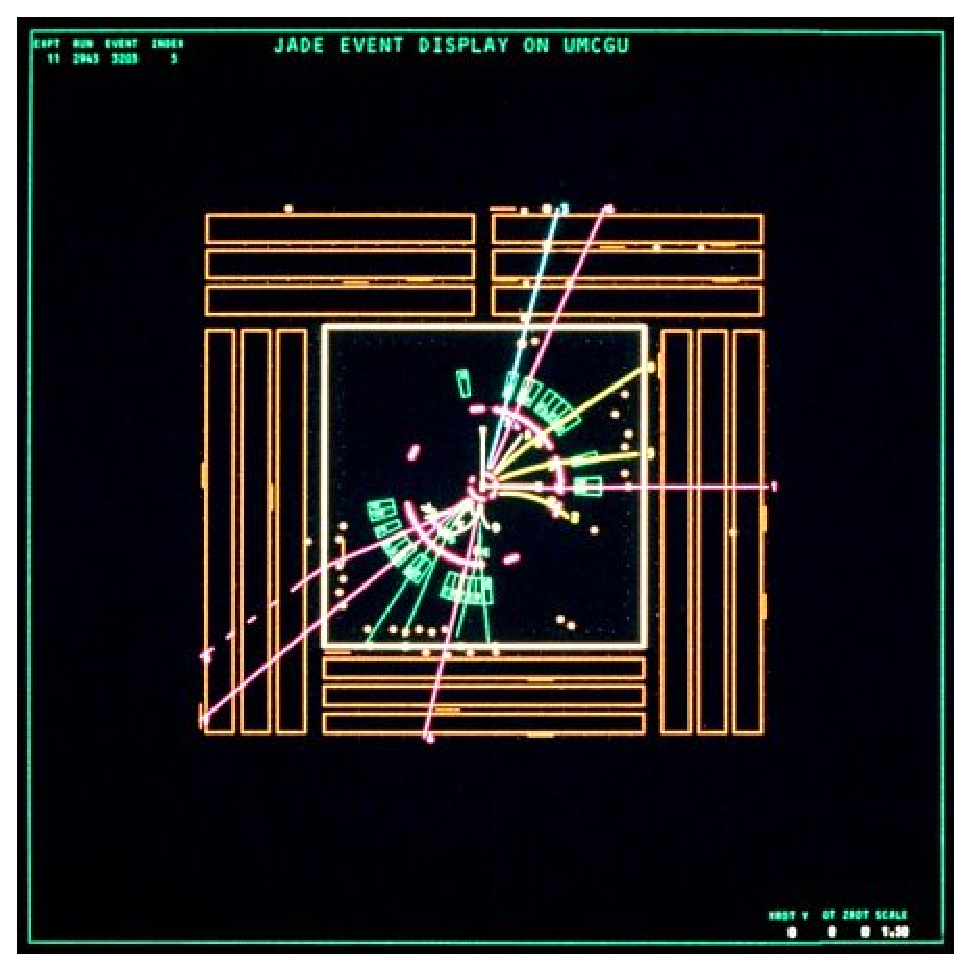
\includegraphics[width=0.36\textwidth]{Figures/display_ref1}\hfill
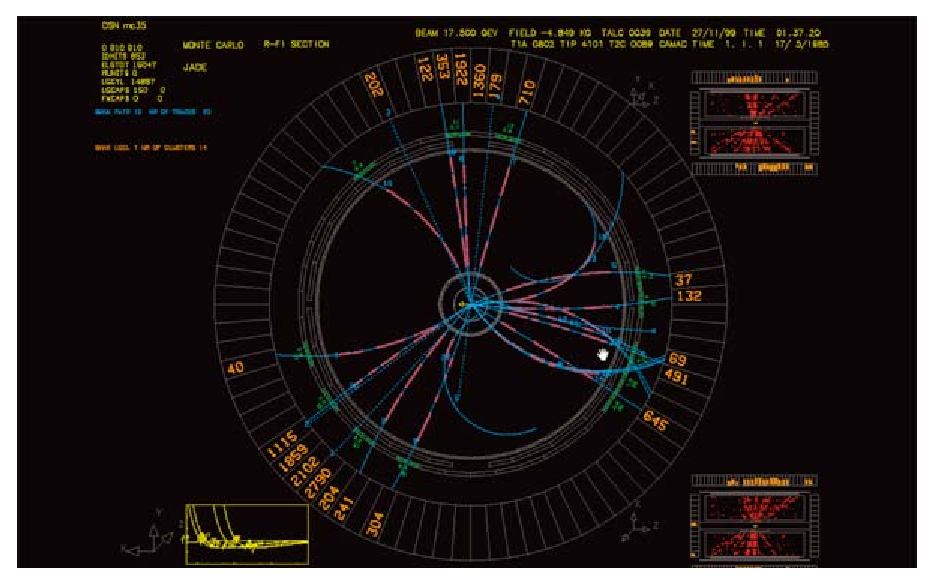
\includegraphics[width=0.58\textwidth]{Figures/display_ref2}
\caption{References: the early display of the JADE experiment (left) and the display of a Monte Carlo event
with the R-$\phi$ section, the lead glass energies and the orthogonal projections (right).}
\label{fig:displayrefs}
\end{figure}
\begin{figure}[H]
\centering
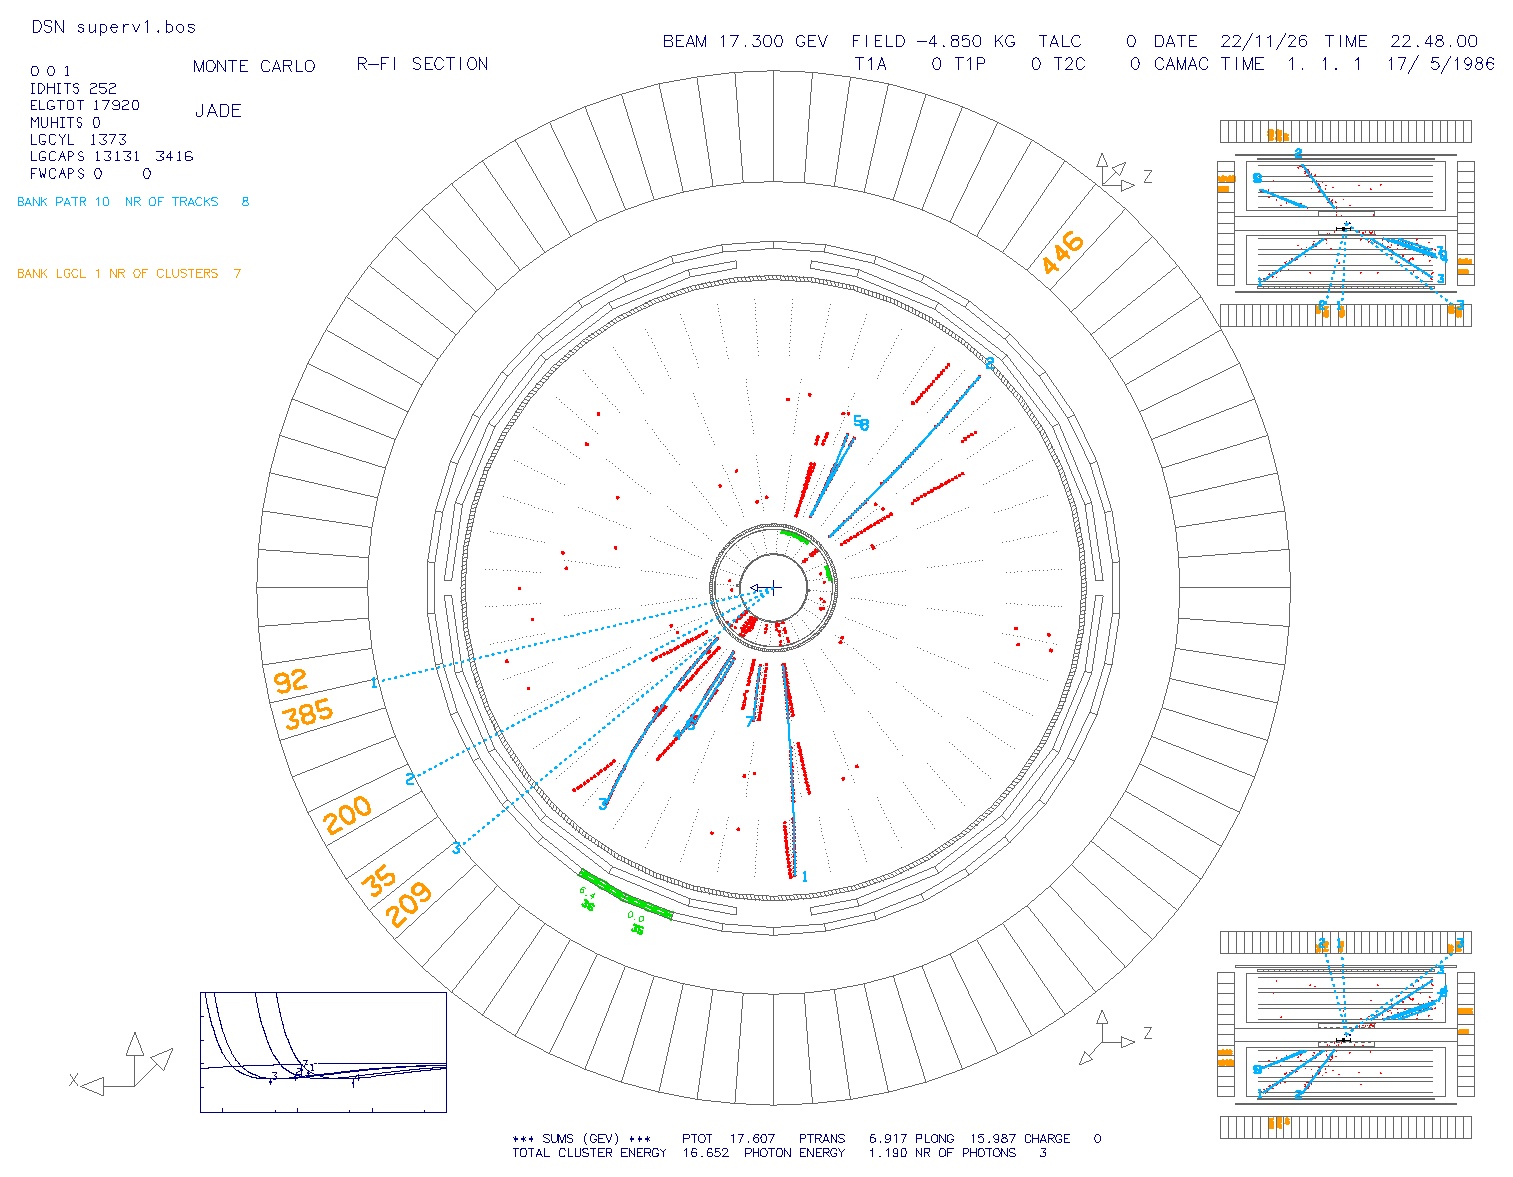
\includegraphics[width=0.48\textwidth]{Figures/display_rphi}\hfill
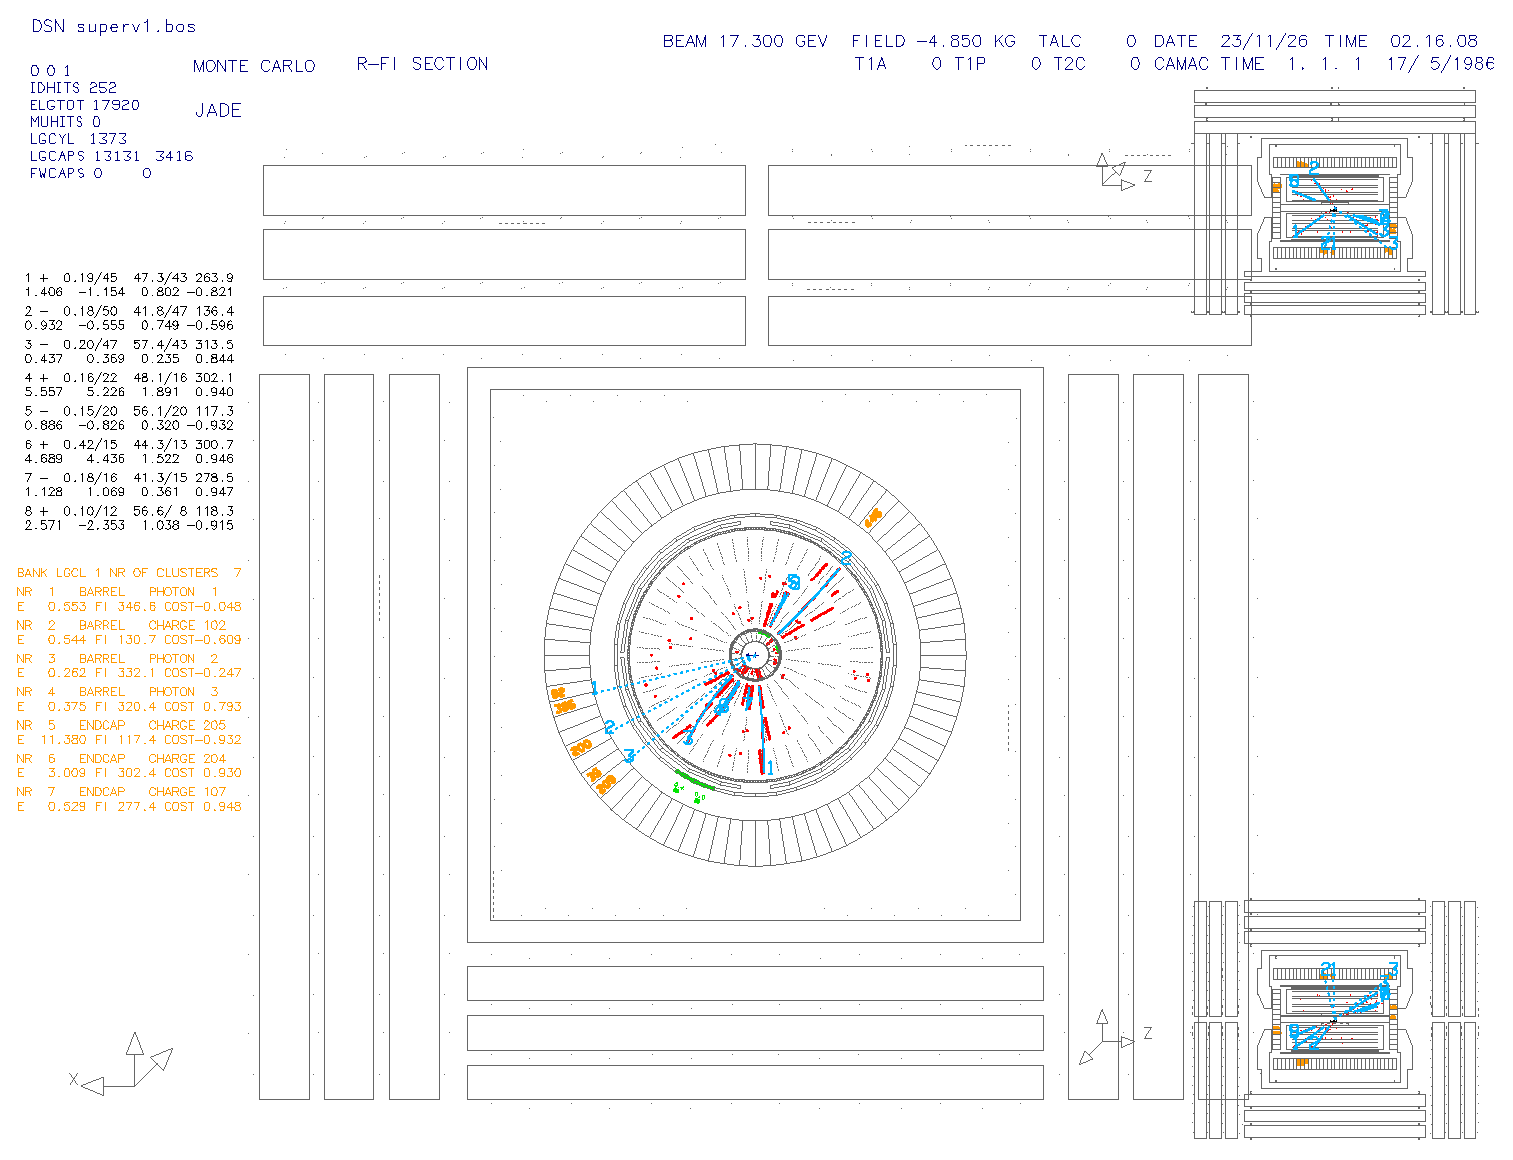
\includegraphics[width=0.48\textwidth]{Figures/display_mc_rc1}
\caption{Pictures written by the event display for a reconstructed Monte Carlo event of the test suite (generated with
Pythia 8): the R-$\phi$ section with the detector hardware, the projections and the dE/dx plot (left), and the hardware view with the
muon chambers and the tables of the tracks and clusters (right). The pictures are not those of the references; they agree in
structure, not pixel by pixel.}
\label{fig:displaytests}
\end{figure}
\FloatBarrier

Not restored compared with the historic pictures are the pink dashed track segments, the filled hit patterns in the
insets of the orthogonal projections (the insets themselves are available with display options 16 and 17), the
letters ``Y'' and ``Z'' of the axis triad and the label of the electron curve of the small dE/dx plot. The
muon chamber hits cannot be shown, since the sample events have no muon hits. An attempt to replace HIGZ by ROOT
graphics (\texttt{picocernlib}, Section~\ref{sec:picocernlib}) was made; it is not the route used: the geometry treatment of ROOT and HIGZ is
conceptually different and the HIGZ behaviour that the display relies on is not documented.

\subsubsection{File catalog}
As the amount of data is small, there is no big need in a complicated file catalogue.
The list of files can be seen online. 


\section{Use of AI in the porting}
\label{sec:ai}

The porting of the software described in this note, from 2016 until November 2026, was done by the maintainer
without AI tools. AI was used only in the last phase, in the week before this version of the note (20--22 November
2026): an AI coding assistant, Claude Code~\cite{ClaudeCode:web}, was used interactively by the maintainer for the
cleanup of the build system, for the porting to new compilers and platforms, for the tests and the continuous
integration, and for the documentation, including this section. The assistant read the code, ran the builds,
tests and debuggers on the machines of the maintainer, proposed and made changes, and wrote drafts of the
documentation. The maintainer defined the tasks, decided what to keep, ran and reviewed the results and committed
the changes. At the request of the maintainer the assistant is listed as a co-author of this note; the maintainer
is responsible for its content. Statements of the assistant were not accepted without a reproduction
(a debugger session, a minimal program or a test). They were wrong in some cases, e.g.\ a description of a change
that mentioned code that was not in the change, a commit placed on the wrong branch, and an overlooked second
byte order problem in the calibration constants (Section~\ref{sec:calfiles}); these were found by review
and by the tests. The following problems were debugged with the help of AI; most of them are old code that
depends on the machine, the compiler or the byte order, and the bugs would have been difficult to see
without a debugger and a systematic comparison.
\begin{description}
\item[Floating point exceptions and different compilers.] The old code divides by zero and produces NaN in a
number of places. It worked with the old compilers because their results were never trapped or because they
differ from the modern ones: Intel \texttt{MAX(0,NaN)} returns the NaN and made the Jacobi iteration of
\texttt{PXDIAM} endless; fused multiply-add of the NVIDIA compiler turned a difference of equal squares into a
small negative number and the square root in \texttt{JELOSS} into a NaN, and the tracking loop did not end; the
NVIDIA compiler treats denormals as zero while the BOS library compares bit patterns kept in real variables
(\texttt{NOTLOW}), so that the memory of the event bank ran out; the preprocessor of the NVIDIA compiler
breaks \texttt{\#} in Hollerith constants. The compiler flags and small changes of the sources were the result.
Intel and NVIDIA also differ in the use of \texttt{ENTRY} dummy arguments, the \texttt{ISNAN} extension,
formatted output of real values with integer edit descriptors and the unit used by the HIGZ PostScript output.
\item[The event display.] The numbers around the calorimeter and the statistics panel were lost, because an early
\texttt{RETURN} was left in \texttt{HEMSYM} and the decoding of the packed stroke font used an
\texttt{EQUIVALENCE} that works only on big-endian machines. The text routine of the PLOT10 emulation
unpacked the last, partial word of the strings in the wrong order on little-endian machines (axis captions,
units, dates). Both were found by comparing the pictures with the historic displays; the display tests check the
colours and the presence of the calorimeter numbers.
\item[A crash of h2root on 64-bit machines.] The converter \texttt{h2root} of ROOT 6.40.04 crashed in about seven
of eight runs. The 64-bit address of the ntuple buffer was passed to Fortran as a 32-bit integer, and the offset
inside the HBOOK store was wrong whenever the upper bits of the address were set, which happens for most
position independent executables. A reproducer with HBOOK files written by CERNLIB was prepared, the bug was
reported and has been fixed in ROOT~\cite{ROOT:hbookfix}; the software now uses the corrected sources.
\item[A bug of the Apple linker.] On macOS the programs failed with segmentation faults and bus errors. The linker
merges the common symbols (the Fortran \texttt{COMMON} blocks) comparing only the lower 16 bits of their sizes, so
that a block larger than 64~KiB gets the size of a small declaration from another object or from CERNLIB.
A minimal reproducer in C and Fortran was written and the bug was reported to Apple. The software uses a
\texttt{BLOCK DATA} unit for each large block, which is compiled only on Apple systems.
\item[Calibration constants that were not applied.] Section~\ref{sec:calfiles}: on little-endian machines the
routine \texttt{KLREAD} skipped all records of the calibration files because of the byte order of the bank
names, and the muon constants needed a correction for integers overlaid on pairs of half-words. The reason
for the missing muon chambers in the display and the warnings of the muon analysis was found in this way. It was
also found that the muon system simulation consists of dummy routines.
\item[Build system and continuous integration.] Changed behaviour of newer CMake versions (the policy
CMP0219 for macro arguments), warnings of the macOS linker about the deployment target, the trust of
Homebrew taps, the restoration of caches that did not contain the X server, the missing check of failed or
skipped tests in the workflows, the reuse of one build directory by different compilers
(Section~\ref{sec:build}) and the 32-bit and aarch64 builds.
\end{description}
The assistant was also used to write and update the descriptions of the changes, the instructions for the
developers (\texttt{AGENTS.md}) and the text of this section; the facts quoted here can be checked in the
history of the repository and in these files.

\section{Data access}
\label{sec:access}

The JADE data can be obtained from the CERN Open Data Portal (Section~\ref{sec:opendata}) and from the storage at MPCDF.
The files of the portal are accessed from the page of the record (\url{https://opendata.cern.ch/record/26999}) and with the
XRootD protocol from the CERN storage (\texttt{root://eospublic.cern.ch//eos/opendata/jade/}); the files of the dataset
are listed in index files, one per directory of the original tapes.

\subsection{Conditions of use of the JADE open data}
The conditions are given by the page ``About JADE'' of the portal, in particular its disclaimer, by the record of the dataset
and by the terms of use of the portal~\cite{CERN:OpenDataTerms}:
\begin{itemize}
\item The JADE dataset, like all datasets and metadata of the portal, is released under the Creative Commons CC0
waiver (the licence of the record is CC0-1.0). The other content of the portal, e.g.\ software, is under its own
licence, and the portal gives its content ``as is''.
\item Neither JADE nor CERN endorse any works, scientific or otherwise, produced with these data.
\item The disclaimer states that all released data samples have a unique DOI that the users are requested to cite in
applications and publications. The record 26999 had no DOI at the time of writing, so that the data are cited
through the number of the record and its address.
\item The record of the author list of the preserved data (record 26050, nine people who took part in the JADE data
preservation after the end of the collaboration: S.~Bethke, O.~Biebel, M.~Blumenstengel, S.~Kluth, J.~Olsson,
P.~Movilla Fernandez, C.~Pahl, J.~Schieck and A.~Verbytskyi) asks that analyses of JADE data from the portal cite this list
together with the data and with the author list of the JADE Collaboration (record 26051, 127 authors, as given in Eur.\
Phys.\ J.\ C73 (2013) 2332).
\item The disclaimer also warns that the data remain complex: selection criteria have to be applied, some understanding
of particle physics and of the detector is required, and the data cannot be viewed in simple tables for
spreadsheet-based analyses.
\end{itemize}
The page ``About JADE'' describes the dataset as events in the BOS format, produced by the reconstruction software, while
the record lists the format as raw; the files with the same names that are used in the test suite are in the FPACK
format and are converted to BOS with \texttt{fptobos} (Section~\ref{sec:data}).

\subsection{Policy of the JADE collaboration}
The draft data preservation policy of the JADE collaboration (\texttt{doc/Policy} of the repository) requires that any
publication that results from the analysis of the data by non-members of the collaboration contains an
acknowledgement that the data were collected by JADE and a disclaimer that the collaboration takes no
responsibility for the results, for example: \emph{``This paper is based on data obtained by the JADE experiment,
but is analyzed independently, and has not been reviewed by the JADE collaboration.''} An analysis can be signed by the
collaboration as a whole after an approval procedure, which consists of an invitation to all members of the
collaboration to take part in the editorial process, and the time between the call and the submission of the
results to a peer-reviewed journal must not be shorter than three months. If a member of the collaboration takes part
in an analysis, it has to be stated whether an approval procedure took place and what its outcome was.

\section{JADE documentation}
Technical notes are available in hard copies and scanned version in MPP (and DESY library?).
Papers are available on InSpire from CERN library or KEK.
The data preservation documentation is available on wwwjade.mpp.mpg.de.
\section{Validation}
The data and MC samples produced in 2003 were reconstructed with JADE2016 software and compared with the 
original reconstructions. Minor differences were found.


\section{Conclusions}
The case of JADE data preservation was studied.

\section*{Acknowledgements}
The author thanks Siegfried Bethke, Richard Hildebrandt, Stefan Kluth, Matthias Schr\"oder,
Ulrich Schwickerath and Tibor \v{S}imko for their help, advice and support of the preservation
of the JADE data and software.
